\documentclass[10pt]{article}

\def\Type{LessonCaelan}
\def\TypeNum{Lesson 16}
\def\TypeTitle{Properties of Definite Integrals  }
\def\Semester{Fall 2021} %Not Used 
\def\Course{MATH 1190 \& 1210}
\def\Targets{  \bf\color{Fuchsia}I2 }

\usepackage{preambleDJ}

%\usepackage{ragged2e}


%%%%%%%%%%%% BEGIN DOCUMENT %%%%%%%%%%%%%%%
%%%%%%%%%%%% BEGIN DOCUMENT %%%%%%%%%%%%%%%
%%%%%%%%%%%% BEGIN DOCUMENT %%%%%%%%%%%%%%%
%%%%%%%%%%%% BEGIN DOCUMENT %%%%%%%%%%%%%%%
%%%%%%%%%%%% BEGIN DOCUMENT %%%%%%%%%%%%%%%




\begin{document}

\pagestyle{otherpages}
\thispagestyle{firstpage}
\vs{.3}

\textbf{Intended Learning Outcomes}
After this lesson, you will be able to 

\begin{itemize}
    \item Interpret, estimate and compute a definite integral geometrically in terms of as the signed area.(\target{I2})
    \item Compute definite integrals using their properties.(\target{I2})
\end{itemize}

\vspace{-0.6cm}

\hrulefill\\

\vspace{-0.6cm}
\important{The Definite Integral}
{
Let $a$ and $b$ be real numbers with $a<b$, and suppose $f$ is continuous on the interval $[a,b]$. The {\bf definite integral} of $f$ from $a$ to $b$ is denoted by \[\int_a^b f(x)\,dx\] and represents the {\it net area} between the graph of $f$ and the interval along the $x$-axis from $a$ to $b$. If $f$ represents the rate of change of a quantity, then $\dint_a^b f(x)\,dx$ represents the {\it net change} in the quantity as $x$ varies from $a$ to $b$.
}


\mpageT{.6}{.4}{
\blue{\bf Signed/Net Area for $\ds \int_a^b f(x)\;dx$}
\itemI{
\item Area of regions above the $x$-axis are {\em positive}
\item Area of regions below the $x$-axis are {\em negative}
}
}{
\begin{flushright}
\begin{tikzpicture}
  \begin{axis}[
%    axis y line = left,
%    axis x line = bottom,
 	axis line style = { line width=1pt},
    xlabel = {$x$},
    ylabel={$y=f(x)$},
    xtick       = {0.5,4.45},
    xticklabels = {$a$ ,$b$ },
    ytick       = {0},
    yticklabels = {},
    samples     = 160,
    domain      = -1:3,
    restrict y to domain=-10:100,
    xmin = -1, xmax = 5,
    ymin = -1.5, ymax = 3,
    width = 3in, height=2in
  ]
  \addplot[name path=f, domain=-1:5,  blue, ultra thick, mark=none, ] {0.5+x*(x-2)*(x-4)/2};
  \path[name path=axis] (axis cs:0,0) -- (axis cs:4.5,0);
\end{axis}
\end{tikzpicture}
\end{flushright}
}
\vs{.3}\\
{\example}\ltrm{\bf\color{Fuchsia}I2}  Compute $\displaystyle\int_{-1}^2 (1-|x|)\ dx$.

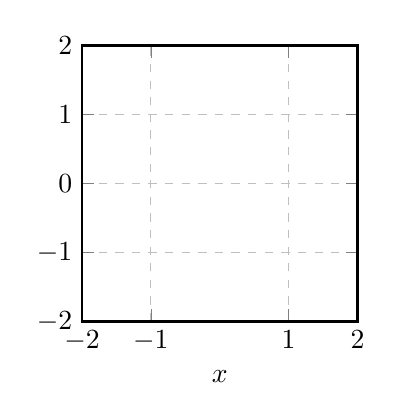
\begin{tikzpicture}
  \begin{axis}[
%    axis y line = left,
%    axis x line = bottom,
 	axis line style = { line width=1pt},
    xlabel = {$x$},
    xtick       = {-3,-2,-1,1,2,3,4,5,6},
    xticklabels = {$-3$,$-2$,$-1$,$1$,$2$,$3$,$4$,$5$,$6$},
    %ytick       = {0},
    %yticklabels = {},
    samples     = 160,
    domain      = -1:3,
    restrict y to domain=-10:100,
    xmin = -2, xmax = 2,
    ymin = -2, ymax = 2,
    width = 2in, height=2in,
    grid=both, grid style=dashed
  ]
\end{axis}
\end{tikzpicture}

\vfill
\newpage
{\exercise}\ltrm{\bf\color{Fuchsia}I2} Compute $\displaystyle\int_0^3(x-1)\ dx$. \\
\mpageT{.25}{.75}{
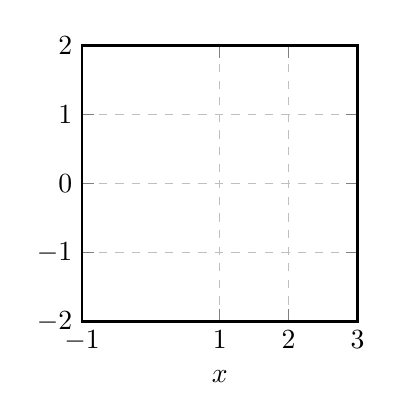
\begin{tikzpicture}
  \begin{axis}[
%    axis y line = left,
%    axis x line = bottom,
 	axis line style = { line width=1pt},
    xlabel = {$x$},
    xtick       = {-3,-2,-1,1,2,3,4,5,6},
    xticklabels = {$-3$,$-2$,$-1$,$1$,$2$,$3$,$4$,$5$,$6$},
    %ytick       = {0},
    %yticklabels = {},
    samples     = 160,
    domain      = -1:3,
    restrict y to domain=-10:100,
    xmin = -1, xmax = 3,
    ymin = -2, ymax = 2,
    width = 2in, height=2in,
    grid=both, grid style=dashed
  ]
\end{axis}
\end{tikzpicture}
}{
\itemC{
\mpageT{.3}{.7}[\hs{.1}]{
\item Graph $f(x)=x-1.$
}{
\item Use common shapes to find the signed (i.e. net) area between $f$ and the $x$-axis on $[0,3]$.
}
}
}

\vfill



{\example}\ltrm{\bf\color{Fuchsia}I2} Use the graph of $f$ below to compute $\dint_{-1}^1 f(x)\,dx$.

\begin{tikzpicture}
  \begin{axis}[
%    axis y line = left,
%    axis x line = bottom,
 	axis line style = { line width=1pt},
    xlabel = {$x$},
    xtick       = {-2,-1,1,2,3,4,5},
    xticklabels = {$-2$,$-1$,$1$,$2$,$3$,$4$,$5$},
        ytick       = {-2,-1,1,2},
    yticklabels = {$-2$,$-1$,$1$,$2$},
    samples     = 160,
    domain      = -1:3,
    restrict y to domain=-10:100,
    xmin = -2, xmax = 5,
    ymin = -2, ymax = 2,
        grid=both, grid style=dashed,
    width = 3.1in, height=2in
  ]
    \addplot[name path=f, domain=-2:5,  blue, ultra thick, mark=none, ] {x<0 ? 1 : (x<1 ? 1-2*x :(  x<2 ? x-2 : (x<4 ? sqrt(1-(x-3)^2)  :4-x )))};
\end{axis}
\end{tikzpicture}


{\exercise}\ltrm{\bf\color{Fuchsia}I2} Use the graph of $f$ above to compute the following definite integrals:
\begin{enumerate}
\item[(a)] $\dint_1^2 f(x)\,dx=$\vs{.1} \\
    ({\it Hint:} the area of a triangle of base $b$ and height $h$ is $A=\dfrac12bh$.)\\

\item[(b)] $\dint_2^4 f(x)\,dx=$ \vs{.1} \\
    ({\it Hint:} the area of a circle of radius $r$ is $A=\pi r^2$.)\\

\item[(c)] $\dint_1^4 f(x)\,dx=$ \vs{.1} \\

\end{enumerate}

\newpage

\important{Definite Integral ``Break Apart" Property}
{
\[\dint_a^b f(x)\,dx = \dint_a^c f(x)\,dx + \dint_c^b f(x)\,dx\]
}



{\exercise}\ltrm{\bf\color{Fuchsia}I2} If $\dint_0^2 g(t)\,dt=4$, $\dint_2^5 g(t)\,dt=-3$, and $\dint_4^5 g(t)\,dt=-1$, then compute the following:\\[0.1in]
\begin{enumerate}
\item[(a)] $\dint_0^5 g(t)\,dt=$\vs{.5} \\

\item[(b)] $\dint_0^4 g(t)\,dt=$  

\end{enumerate}
\vfill
\begin{minipage}[t]{0.55\textwidth}
{\bf\color{blue}Extra Practice 1.}\ltrm{\bf\color{Fuchsia}I2} Sketch the graph of a continuous function $g$ satisfying all the integral equations in Exercise C. {\em Hint:} Consider using common objects with known area formulas (e.g. rectangles, triangles, etc.).
\end{minipage}
%
\hfill
%
\begin{minipage}[t]{0.4\textwidth}
\,\\[-0.1in]
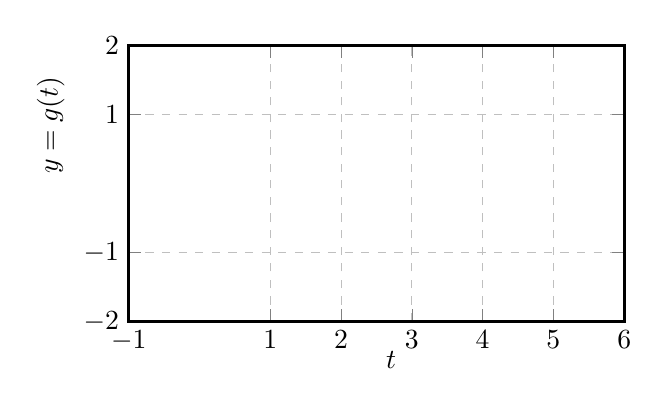
\begin{tikzpicture}
  \begin{axis}[
%    axis y line = left,
%    axis x line = bottom,
 	axis line style = { line width=1pt},
    xlabel = {$t$},
    xtick       = {-1,1,2,3,4,5,6},
    xticklabels = {$-1$,$1$,$2$,$3$,$4$,$5$,$6$},
        ytick       = {-2,-1,1,2},
    yticklabels = {$-2$,$-1$,$1$,$2$},
    ylabel ={$y=g(t)$},
    xlabel style = {anchor= west},
    ylabel style = {anchor=south west},
    samples     = 160,
    domain      = -1:3,
    restrict y to domain=-10:100,
    xmin = -1, xmax = 6,
    ymin = -2, ymax = 2,
        grid=both, grid style=dashed,
    width = 3.1in, height=2in
  ]
\end{axis}
\end{tikzpicture}
\end{minipage}

\vfill
\newpage

\important{Definite Integral ``Reverse Limits" Property}
{
\[\dint_a^b f(x)\,dx = -\dint_b^a f(x)\,dx\]
}

{\exercise}\ltrm{\bf\color{Fuchsia}I2} Use the graph of $f$ below to compute the given integrals. {\small({\it Hint:} reuse work in Exercise B!)}\\
\vs{-.3}
\mpageT{.4}{.6}[\hs{.1}]{
\begin{tikzpicture}
  \begin{axis}[
%    axis y line = left,
%    axis x line = bottom,
 	axis line style = { line width=1pt},
    xlabel = {$x$},
    xtick       = {-1,1,2,3,4,5,6},
    xticklabels = {$-1$,$1$,$2$,$3$,$4$,$5$,$6$},
        ytick       = {-2,-1,1,2},
    yticklabels = {$-2$,$-1$,$1$,$2$},
    ylabel ={$y=f(x)$},
        xlabel style = {anchor= west},
    ylabel style = {anchor=south west},
    samples     = 160,
    domain      = -1:3,
    restrict y to domain=-10:100,
    xmin = -1, xmax = 6,
    ymin = -2, ymax = 2,
        grid=both, grid style=dashed,
    width = 3.1in, height=2in
  ]
    \addplot[name path=f, domain=-2:5,  blue, ultra thick, mark=none, ] {x<0 ? 1 : (x<1 ? 1-2*x :(  x<2 ? x-2 : (x<4 ? sqrt(1-(x-3)^2)  :4-x )))};
\end{axis}
\end{tikzpicture}
}{
(a) $\dint_2^1 f(x)\,dx=$\\[0.2in]
(b) $\dint_4^2 f(x)\,dx=$\\[0.2in]
(c) $\dint_4^1 f(x)\,dx=$\\[0.2in]
}

\newpage

\vs{.35}
\important{Definite Integral ``Linearity" Properties}
{
\[\dint_a^b cf(x)\,dx = c\dint_a^b f(x)\,dx \quad\text{ and }\quad \dint_a^b(f(x)\pm g(x))\,dx = \dint_a^b f(x)\,dx \pm \dint_a^b g(x)\,dx\]
}

{\exercise}\ltrm{\bf\color{Fuchsia}I2} The graph of $f$ is given below. We don't know the graph of $g$, but suppose we do know $\dint_0^2 g(x)\,dx = \pi$ and $\dint_2^4 g(x)\,dx=-\pi$. Compute the following integrals.

\mpageT{.4}{.6}[\hs{.1}]{
\vspace{-0.1in}
\begin{tikzpicture}
  \begin{axis}[
	axis line style = { line width=1pt},
	xlabel = {$x$},
	xtick       = {-1,1,2,3,4,5,6},
    	xticklabels = {$-1$,$1$,$2$,$3$,$4$,$5$,$6$},
        ytick       = {-2,-1,1,2},
    	yticklabels = {$-2$,$-1$,$1$,$2$},
    	ylabel ={$y=f(x)$},
        xlabel style = {anchor= west},
    	ylabel style = {anchor=south west},
    	samples     = 160,
    	domain      = -1:3,
    	restrict y to domain=-10:100,
    	xmin = -1, xmax = 6,
    	ymin = -2, ymax = 2,
        grid=both, grid style=dashed,
    	width = 3.1in, height=2in
  ]
    \addplot[name path=f, domain=-1:6,  blue, ultra thick, mark=none, ] {x<2 ? -(4-x^2)^(1/2) :  (x<4 ? sqrt(1-(x-3)^2)  : 4-x )};
  \path[name path=axis] (axis cs:-1,0) -- (axis cs:6,0);
\end{axis}
\end{tikzpicture}
}{
(a)   $\displaystyle\int_0^2 (f(x)-g(x))\,dx$
}
\begin{enumerate}
\item[(b)] $\displaystyle\int_2^4 (f(x)-g(x))\,dx$
    \vs{.5}

\item[(c)] $\displaystyle\int_0^4 (f(x)-g(x))\,dx$
\vs{.5}

\item[(d)] $\displaystyle\int_4^0 2(f(x)-g(x))\,dx$
    \vfill
\end{enumerate}

\newpage

{\exercise}\ltrm{\bf\color{Fuchsia}I2} Use the graph of $f$ below to highlight a region that could represent the integral below. Find the value of the integral. \vs{-.1}\\
%\vs{-.3}
\mpageT{.4}{.6}[\hs{.1}]{
\begin{tikzpicture}
  \begin{axis}[
%    axis y line = left,
%    axis x line = bottom,
 	axis line style = { line width=1pt},
    xlabel = {$x$},
    xtick       = {-1,1,2,3,4,5,6},
    xticklabels = {$-1$,$1$,$2$,$3$,$4$,$5$,$6$},
        ytick       = {-2,-1,1,2},
    yticklabels = {$-2$,$-1$,$1$,$2$},
    ylabel ={$y=f(x)$},
        xlabel style = {anchor= west},
    ylabel style = {anchor=south west},
    samples     = 160,
    domain      = -1:3,
    restrict y to domain=-10:100,
    xmin = -1, xmax = 6,
    ymin = -2, ymax = 2,
        grid=both, grid style=dashed,
    width = 3.1in, height=2in
  ]
      \addplot[name path=f, domain=-2:5,  blue, ultra thick, mark=none, ] {x<0 ? 1 : (x<1 ? 1-2*x :(  x<2 ? x-2 : (x<4 ? sqrt(1-(x-3)^2)  :4-x )))};
  \path[name path=axis] (axis cs:-2,0) -- (axis cs:5,0);
    %\draw[ultra thick, red] (3,0)--(3,1);
\end{axis}
\end{tikzpicture}
}{
$\ds \int_3^3 f(x)\,dx=$\\
}

\important{Definite Integral ``Area of a Line Segment" Property}
{
\[\dint_a^a f(x)\,dx = 0\]
}

The following problem was adapted from a problem appearing on an assessment during the Fall 2023 semester.

{\bf\color{blue}Exam Practice 2.}\ltrm{\bf\color{Fuchsia}I2} Given $\displaystyle \int_{3}^{-2} f(x)\,dx=1$, $\displaystyle \int_{0}^3 f(x)\,dx = 2$, and $\displaystyle\int_{-2}^3 \left(2f(x)-g(x)\right)\,dx=3$, evaluate the following using properties of definite integrals: 
\enumA{
    \item $\displaystyle\int_{-2}^3 f(x)\,dx$\\[0.5in]
    
    \item $\displaystyle\int_{-2}^0 f(x)\,dx$
        \vfill
    \item $\displaystyle\int_{-2}^3 g(x)\,dx$
        \vfill
}

\end{document}
